\documentclass[12 pt,twopage]{article}
\usepackage{amsmath,amssymb,amsfonts,amsthm}
\usepackage[english]{babel}
\usepackage[utf8]{inputenc}
\usepackage{fancyhdr}
%\usepackage[a3paper]{geometry}
\usepackage{geometry}
\usepackage{tikz}
\usepackage{xcolor}
\usepackage{float}
\usepackage{bm}
\usepackage{listings}
\usepackage{xcolor}
\usepackage{algorithm2e}
\usepackage{tikz}
\usetikzlibrary{automata,positioning}

\lstset{basicstyle=\ttfamily,
 showstringspaces=false,
 commentstyle=\color{gray},
 keywordstyle=\color{blue},
 morekeywords={grep, head, tail, cut }
}

\newcommand{\codepath}{../}
\newcommand{\scriptpath}{../scripts}

\newcommand{\hr}{\begin{center} \line(1,0){450} \end{center}}
\newcommand{\R}{\mathbb R}
\newcommand{\B}{ \{0,1\} }
\newcommand{\tr}{^\mathsf{T}}
\newcommand{\F}{\mathcal{F}}
\newcommand{\norm}[1]{\left\lVert#1\right\rVert}
\DeclareMathOperator{\Id}{Id}
\DeclareMathOperator{\diag}{diag}
\DeclareMathOperator{\epi}{epi}
\DeclareMathOperator{\co}{co}
\DeclareMathOperator{\interior}{int}
\DeclareMathOperator{\Proj}{Pr}
\DeclareMathOperator*{\argmin}{argmin}
\DeclareMathOperator*{\argmax}{argmax}
\newcommand{\midd}{\mathrel{}\middle|\mathrel{}}


\newcommand{\generalPdfSymbol}{\bm{p}}
\newcommand{\gps}{\generalPdfSymbol}
\newcommand{\bernoulliPdfSymbol}{p_{bern}}
\newcommand{\binomialPdfSymbol}{p_{bin}}

\newcommand{\s}[1]{\sum_{#1}}
\newcommand{\am}[2]{\argmax\limits_{#1} #2}
\newcommand{\partition}[2]{\{ #1_1, #1_2, \dots, #1_{#2} \} }
\newcommand{\pd}[2]{#1 \left( #2 \right) }
\newcommand{\p}[1]{\pd{P}{#1}}
\newcommand{\cp}[3]{\pd{#1}{#2 \midd #3}}
\newcommand{\cpf}[3]{ \frac{\pd{#1}{#2,#3}} { \pd{#1}{#3} } }
\newcommand{\cpeq}[3]{\cp{#1}{#2}{#3} = \cpf{#1}{#2}{#3}}

\newcommand{\ltp}[3]{\s{#2_j \in \partition{#2}{n} } \cp{#1}{#3}{#2_j} \p{#2_j} }
\newcommand{\bysNom}[3]{\cp{#1}{#3}{#2_i} \pd{#1}{#2_i} }
\newcommand{\bys}[3]{ \frac{\bysNom{#1}{#2}{#3} }{ \ltp{#1}{#2}{#3} } }
\newcommand{\byseq}[3]{}


\newcommand{\bernoulli}[2]{ #1^{#2} \left(1 - #1\right)^{1 - #2}  }
\newcommand{\bern}{\bernoulli{\phi}{c}}

\newcommand{\likelihood}[1]{\prod\limits_{c \in C} #1 }


%\geometry{top=20mm, left=20mm, right=10mm, bottom=15mm}

\pagestyle{fancy}
\lhead{Christian Lengert 153767}
\rhead{\today}
\chead{Latent Dirichlet Allocation}
%\rfoot{Page \thepage}

 \setlength{\parindent}{0pt}
\begin{document}

\begin{abstract}

 In this article we will explore the model of Latent Dirichlet Allocation theoretically by introducing the model and multiple algorithms for model selection and inference and practically by implementing an inference algorithm based on Gibb's sampling and exploring and visualizing the results.
 The first section will give an overview about the model and the domain of problems it is applied to.
 The second section explains a way to implement the model-selection algorithm in Python and a simple approach to parallelize the inference process.
 In the third section we will train a model on a subset of the simple english Wikipedia and evaluate the results by visualizing the learned topics with the Python library pyLDAviz.
\end{abstract}
%\twocolumn
\section{Latent Dirichlet Allocation}
The model of Latent Dirichlet Allocation (LDA) is a generative probabilistic model for collections of discrete data proposed by Blei, Ng and Jordan \cite{Blei2003}. It is a mixture model that tries to model latent topics or concepts of multinomial observations, e.g. words in text corpus.
\begin{figure}[h]
 \begin{center}
  \begin{footnotesize}
   \begin{description}
    \item[\( K \)] : Number of topics to be found by the model
    \item[\( M \)] : Number of documents in the corpus
    \item[\( V \)] : Number of unique terms in the dictionary
    \item[ term \(t\)] 
    \item[\( \vec\alpha \in \mathbb{R}^K \)] : Hyperparameter of the document-topic Dirichlet distribution
    \item[\( \vec\beta \in \mathbb{R}^V \)] : Hyperparameter of the topic-word Dirichlet distribution
    \item[\( \vec\vartheta_m \in \mathbb{R}^K \)] : Topic distribution of each document \(m\).
    \item[\( \vec\phi_k \in \mathbb{R}^V \)] : Term distribution of each topic \(k\).
    \item[\( N_m \)] : The length of the m-th document.
    \item[\( z_{m,n} \)] : Topic index for the \(n\)-th word in document \(m\).
    \item[\( w_{m,n} \)] : the \(n\)-th word in document \(m\).
   \end{description}
  \end{footnotesize}
 \end{center}
 \caption{Notation}
 \label{fig:notation}
\end{figure}

%To understand the structure of the model we will look at the Likelihood-function for
%The probability of a term to occur in a document \(p \left( w=t \right)\) is modeled as a marginal distribution %of the joint distribution over topics and terms.
%\onecolumn
%%\begin{equation}
%% p\left( w=t \right) = \sum\limits_{k} p\left( w=t \midd z=k \right) p\left( z=k \right)
%%\end{equation}
%
%\begin{equation*}
% p\left( \vec{w}_{m}, \vec{z}_{m}, \vec{\vartheta}_{m} \midd \vec{\alpha}, \vec{\beta} \right) = %\prod\limits_{w_{m,n}}^{N_m} p \left(w_{m,n} \midd \vec\phi_{z_{m,n}} \right) p \left(z_{m,n} \midd %\vec\vartheta_{m} \right) p\left( \vec\vartheta_m \midd \vec\alpha \right) p \left( \phi \midd \vec\beta \right)
%\end{equation*}

%bag of words
%documents plate
%corpus plate
\subsection{Generative Process}
To understand the model we analyze the LDA generative model, of which an implementation is in the appendix \ref{code:generativeModel}. To generate a corpus consisting of multiple documents, the steps shown in figure \ref{fig:generativeProcess} have to be taken.

Given the number of topics \(K\), the number of documents \(M\), the Dirichlet-hyperparameters \(\alpha,\beta\) and the moment of the Poisson distribution \( \xi \) we start by specifiying the topics by sampling a categorical topic-word distribution \(\phi_k \) for every topic. These hold a probability for every possible term to occur in the context of the topic. We sample the topic-categoricals from a Dirichlet distribution with the parameter \(\beta\).

With the Dirichlet-samples we can start to generate documents. For every document \( d \) we sample from a Dirichlet distribution again, this time using with the hyperparameter \( \alpha \). The resulting categorical distribution sets probabilities for all topics to be included in the documents. Furthermore we sample a document length from the Poisson distribution.

Finally, for every word to be generated, we sample a topic index from the documents associated document-topic-categorical distribution and then sample the term given the topics multinomial distribution.
\onecolumn
\begin{figure}
 \begin{center}
  \begin{algorithm}[H]
   \KwData{Number of topics \(K\), Number of Documents \(M\), Dirichlet parameters \(\alpha\) and \(\beta \), Poisson parameter \(\xi\)}
   \KwResult{Corpus \( c \)}
   \For{all topics \(k \in [1,K] \) }{
    sample topic-term distribution parameters \( \phi_k \sim Dir \left( \beta \right) \)
   }
   \For{ all documents \( m \in [1,M] \)}{
    sample document-topic distribution parameters \( \vartheta \sim Dir \left( \alpha \right) \)\\
    sample document-length \(l_m \sim Poisson \left( \xi \right) \)\\
    \For{ all words \( w \in [1,l_m] \)}{
     sample topic index \( z_{m,n} \sim Mult\left( \xi \right)\)\\
     sample term for word \( w_{m,n} \) from \( p\left( w_{m,n} \midd z_{m,n}, \beta \right)\) \( w_{m,n} \sim Mult\left( \phi_{z_{m,n}} \right) \)
    }
   }
   
  \end{algorithm}
  \caption{The generative model of LDA  \cite{Blei2003,Heinrich2005}}\label{fig:generativeProcess}
 \end{center}
\end{figure}
\subsection{Inference Algorithm}\label{sec:inference}
Various algorithms to tackle the inference problem for LDA have been proposed \cite{Blei2003}. In this report we will focus on a specific Markov-Chain Monte-Carlo based method, namely a Gibb's sampler. We will infere with the algorithm explained by Pefta et. al. of which an overview can be found in figure \ref{fig:algorithm}.

We will use the following formulas to compute the multinomial parameters given the
How to a
\begin{figure}
 \begin{center}
  \begin{algorithm}[H]
   \KwData{Word vectors \( \{ \vec{w} \} \), Number of Documents \(M\), Dirichlet parameters \(\alpha\) and \(\beta \), Number of topics \(T\)}
   \KwResult{topic associations \( \{ \vec{z} \} \)}
   Initialize count variables \( n_m^{(k)} ,n_m, n_k^{(t)}, n_k \)\\
   Initialize multinomial parameters \(p_t\)
   \For{all documents \( m \in [1,M] \) }{
   \For{all wordpairs \( (i,c) \in m \) }{
    \For{all occurences \(c\) of a term \(i\) }{
     sample topic index \(z_{m,n} = k \sim Mult\left( 1/K \right)\)\\
     increment document-count: \(n^{(k)}_m += 1\)\\
     increment document-sum: \(n_m += 1\)\\
     increment topic-count: \(n^{(t)}_k += 1\)\\
     increment topic-sum: \(n_k += 1\)
    }}
   Gibb's sampling:\\
   \For{ all iterations }{
   \( n_m^{(k)} -= 1; n_m -= 1; n_k^{(t)} -= 1; n_k -= 1; \)\\
   sample \( z_{m,n} = \overline{k} \sim p\left( z_i \midd \vec{z}_{\neg i} \right) \) \\
   \( n_m^{(\overline{k})} -= 1; n_m -= 1; n_{\overline{k}}^{(t)} -= 1; n_k -= 1; \)
   }
   }
   
  \end{algorithm}
  \caption{A variational inference algorithm \cite{Heinrich2005}}\label{fig:algorithm}
 \end{center}
\end{figure}


%describe algorithm
%what are hyperparameteres
%what are cojugate priors
\section{Implementation}
Although the inference algorithm can potentially be parallelized in multiple ways \cite{Newman2006ScalablePT,Wang2009PLDAPL}, we aim to create a serial implementation for to strive for correctness instead of performance.
\subsection{Preparation}
First we have to choose a text corpus to estimate the parameters of the LDA-model from. For this we use an instance of the simple english Wikipedia \cite{simplewi84:online}, the version 'All pages, current versions only'.

For the purpose of speeding up the development process we will perform our operations on an even smaller subset of only 5 articles, to avoid long loading times on every run. We split some articles of the downloaded file into a smaller file with the script in section \ref{extract}.

\subsection{Class : Dataset}
We aggregate all operations regarding the preprocessing of the corpus in a class named Dataset, which can be examined in section  \ref{class:dataset}. Our goal is to load and parse the XML-file, select the relevant parts of each article, apply linguistic preprocessing to the articles, count the occuring words and build a dictionary. After the processing by our class we want to have a list of lists of pairs \((t,c)\), where \(t\) is a term-index and \(c\) is the count of instances of a term in a document, as well as a dictionary with all terms.


\paragraph{Parsing XML}  To parse the XML-file we add the member-function \texttt{loadXMLFile} and utilize the the native Python \texttt{xml} module, that allows us to extract the articles with just one expression.
\paragraph{Linguistic Preprocessing} To prepare the text we use the function \texttt{preprocess\_string} from the package \texttt{gensim} as it does performs all needed operations in one step. As this function can be applied to every document independently it qualifies to be executed in parallel. We exploit this using the \texttt{multiprocessing} package.
With using \texttt{preprocess\_string} we perform the following operations:

\begin{enumerate}
 \item Remove the syntactic constructs of the Wikipedia markup language
 \item Strip punctuation
 \item Remove multiple whitespaces
 \item Drop numeric words
 \item Remove stopwords
 \item Strip words shorter than three characters
 \item Apply stemming
\end{enumerate}
\paragraph{Building a dictionary} As a dictionary we use the class \texttt{dictionary} from the \texttt{gensim}-submodule \texttt{corpora.dictionary} which provides us the possibility to efficiently build a dictionary and map from words to the term-index and back utilizing Python-dictionaries.
\paragraph{Counting words} As final step we count the occurences of terms in a document and construct the list of lists of pairs. This decreases the size of the in memory significantly and can be speed up by using \texttt{multiprocessing} again. Furthermore we choose to drop all Documents with less than four terms.
\paragraph{Utilities} For convenience we add functions to load and restore a dataset to Python-serialization format \texttt{pickle}, to avoid redoing the previous steps on every startup.



\subsection{Class : LDA}
This class holds two verisions of the inference algorithm
\subsubsection{Serial Algorithm}
The serial infernce algorithm from section \ref{sec:inference} is implemented in the function \texttt{fit}.
\subsubsection{Simple Parallelization}
To parallelize the inference process we introduce the function \texttt{fitParallel} which only adds the parameter of the number of used processing cores to the signature of \texttt{fit}. To allow multiple threads to access the datastructures of the model all of them need to be in the global namespace. Therefore we publish them with the  \texttt{global} keyword. Note that this is not a good programming practice as manipulating global state from inside an objects member-function strongly violates the principle of encapsulation and is a severe side-effect. Nonetheless, this allows us to speed up the inference process with very low effort and our model is for exploration only and it is not planned to be used in production.

We parallelize the loop over all documents so that in each iteration we process all documents in parallel.
Apart from making the structures publicly available we have to ensure that access to the count variables is locked. We decrease the document-topic- and topic-term counts, as well as the corresponding sum-structures before sampling a new topic index and increase them afterwards. In this, the topic-term structures could possibly accessed by multiple threads at once. This can lead to race conditions where threads read the wrong counts which leads again to a faulty parameter estimation. We avoid this by introducing locks for terms and topics, that ensure unique access.

\section{Evaluation}
To evaluate the topics that the model has learned in the training process on the wikipedia dataset we will use the Python package PyLDAviz. All plots show an intertopic distance map on the left side and a histogram on the right side. The distance map is a two dimensional projection of the topic space computed with a multidimensional scaling algorithm \cite{Sievert2014}. The Histogram shows the most frequent terms for the chosen topic in descending order, in which the the red bar shows the term frequency in the topic and the blue bar the overall term frequency. We will look at the results of a model trained with the parallel algorithm..

\subsection{Performance}
The measurements where taken on a machine with four AMD Opteron 6174 processors with 12 cores each.
\paragraph{Dataset}
Parsing the full XML-file and preprocessing the text took \(126.12\) seconds and computing the term-count pairs took \(126.5174\) seconds resulting in a corpus with \(144337\) documents and \(421397\) terms. Storing the corpus serialized consumes about \(127\) mb.
\paragraph{Inference}
The model in use is trained for 500 iterations  on a subset of the whole corpus of \( 196934 \) documents with \( 752612 \) unique terms which took about \(10\) hours.
\section{Learned Topics}
Finally we can evalute the learned topics, plots created with \texttt{pyLDAvis} are included figures \ref{fig:m2t12}, \ref{fig:m2t34} and \ref{fig:m2t56}.
\paragraph{Topic 1} contains many terms related to the governmental activities of countries and yearly statics of economy. Representative terms are \enquote{population},\enquote{gdp},\enquote{year},\enquote{rank} and \enquote{establish}.
\paragraph{Topic 2}  consists of terms  related to internet, communcation and publication. The five most frequent terms are \enquote{http}, \enquote{title},\enquote{url},\enquote{web} and \enquote{cite}.
\paragraph{Topic 3} intersects with the first topic in the distance map. Indeed it shares the stems of \enquote{population}, \enquote{government}, \enquote{leader} and \enquote{capital} but lacks terms related to the economy.

\paragraph{Topic 4} seems to be related to american motion picture industry and actors. Frequent terms are \enquote{movie},\enquote{american}, \enquote{award} and \enquote{best}. Less frequent are \enquote{season},the stem of \enquote{series} and \enquote{star}.
\paragraph{Topic 5} is related to rock music with \enquote{music}, \enquote{rock} and \enquote{record} as most frequent terms and to the makings of a band in terms of personnel with \enquote{group}, \enquote{member} and \enquote{singer}.
In the distance map we can see a possible intersection, at least a low relative distance to the fourth topic. This makes sense as both topics are related to entertainment, art and public media.

\paragraph{Topic 6} has \enquote{people}, \enquote{word}, \enquote{mean},\enquote{differ} and \enquote{like} and \enquote{us} as most frequent terms. This points to communcation of intentions between people and evalution.


\begin{figure}
 \begin{subfigure}[c]{1\textwidth}
  \caption{Topic 1}
  \centering
  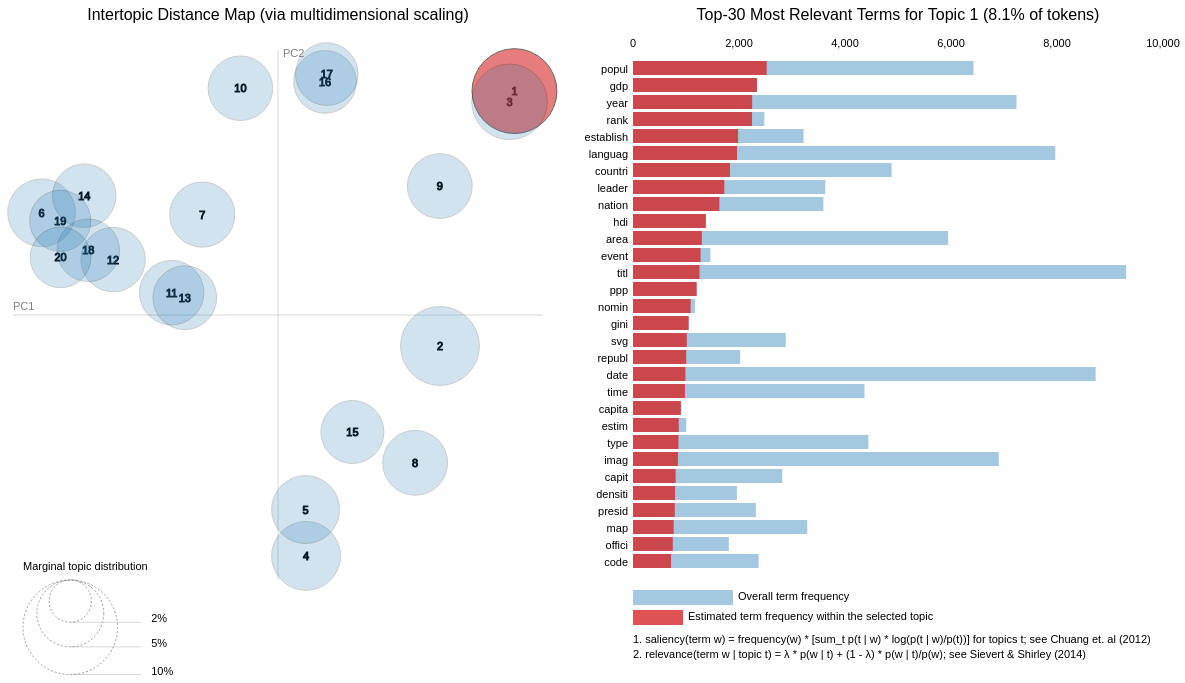
\includegraphics[width=.9\linewidth]{\gpath/m2t1.png}
 \end{subfigure}
 \begin{subfigure}[c]{1\textwidth}
  \caption{Topic 2}
  \centering
  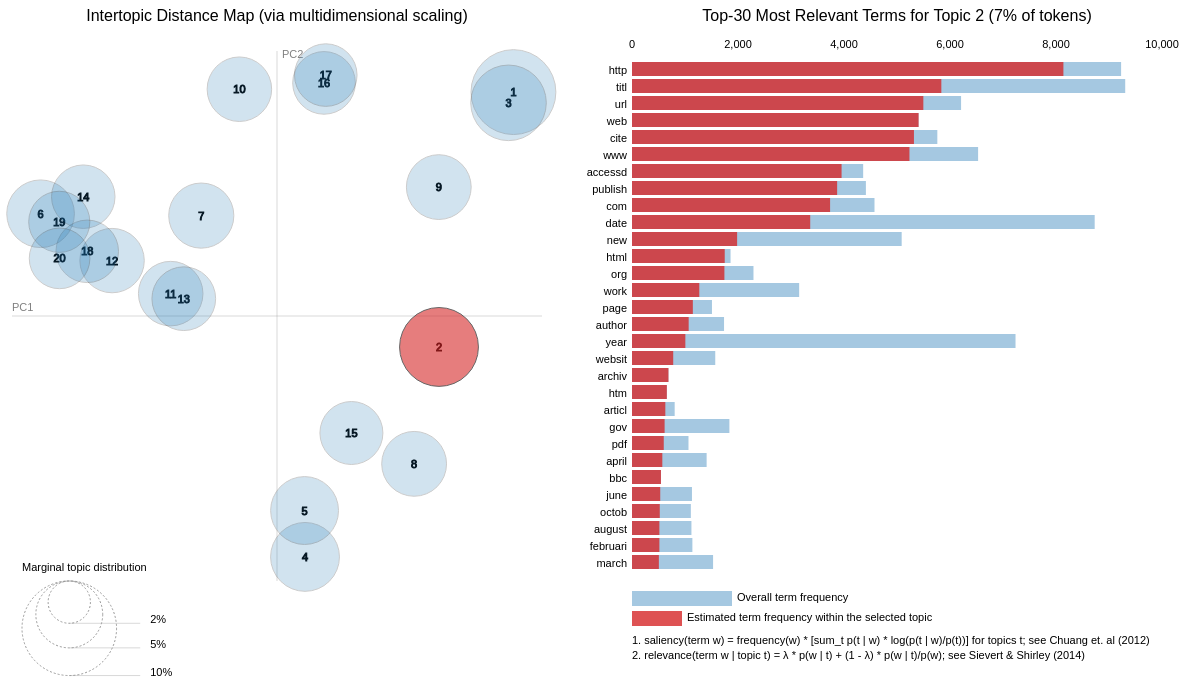
\includegraphics[width=.9\linewidth]{\gpath/m2t2.png}
 \end{subfigure}
 \caption{Plots of the first six topics}
 \label{fig:m2t12}
\end{figure}


\begin{figure}
 \begin{subfigure}[c]{1\textwidth}
  \caption{Topic 3}
  \centering
  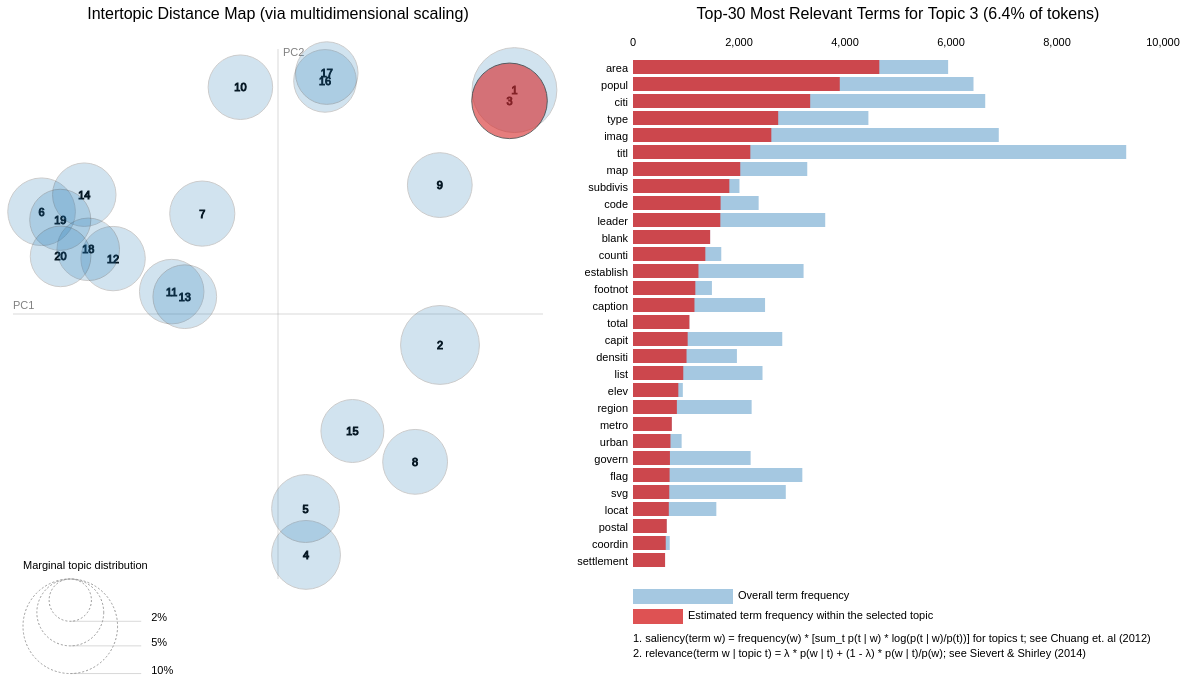
\includegraphics[width=.9\linewidth]{\gpath/m2t3.png}
 \end{subfigure}
 \begin{subfigure}[c]{1\textwidth}
  \caption{Topic 4}
  \centering
  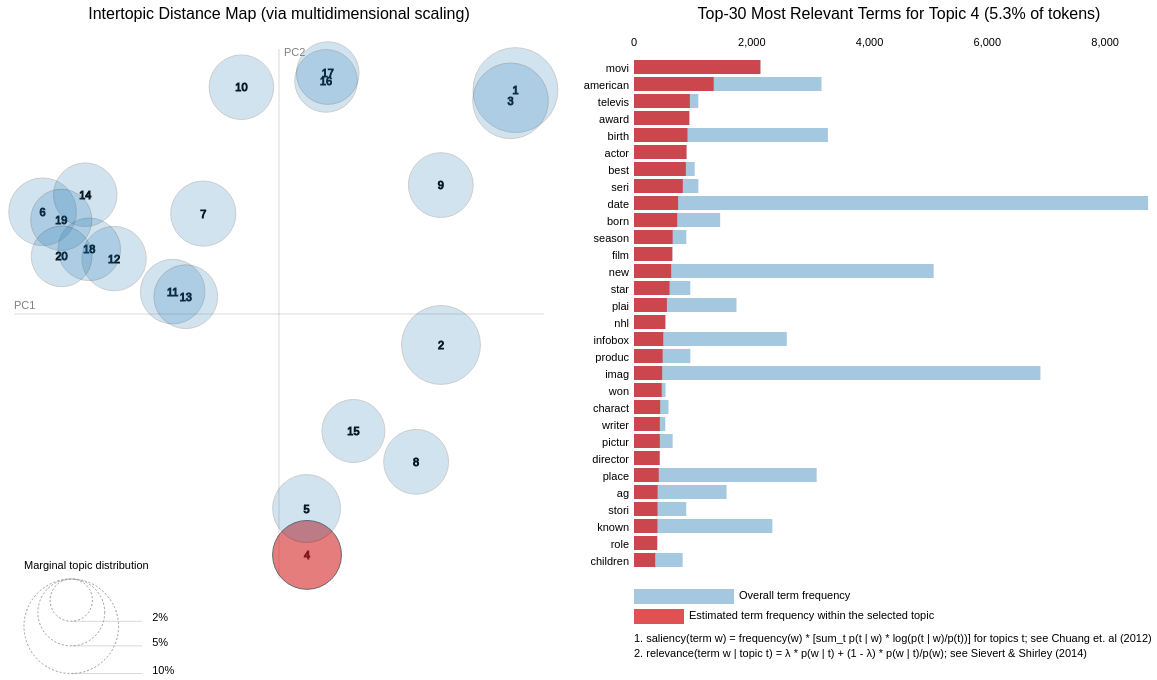
\includegraphics[width=.9\linewidth]{\gpath/m2t4.png}
 \end{subfigure}
 \caption{Plots of topic 3 and 4}
 \label{fig:m2t34}
\end{figure}


\begin{figure}
 \begin{subfigure}[c]{1\textwidth}
  \caption{Topic 5}
  \centering
  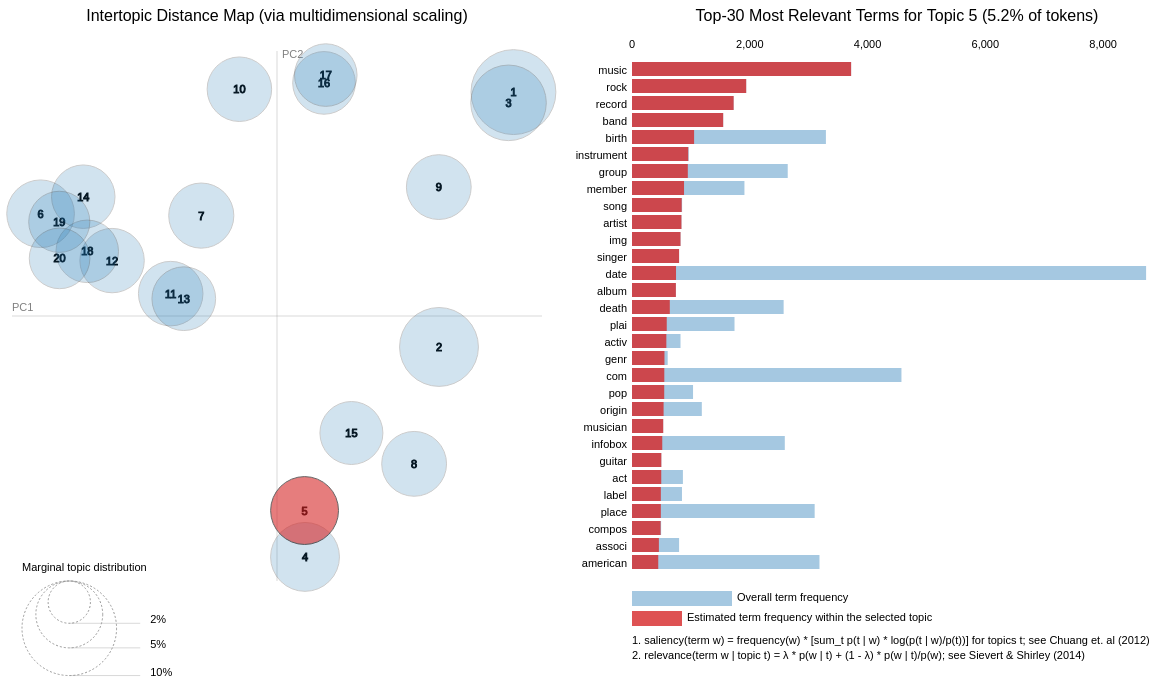
\includegraphics[width=.9\linewidth]{\gpath/m2t5.png}
 \end{subfigure}
 \begin{subfigure}[c]{1\textwidth}
  \caption{Topic 6}
  \centering
  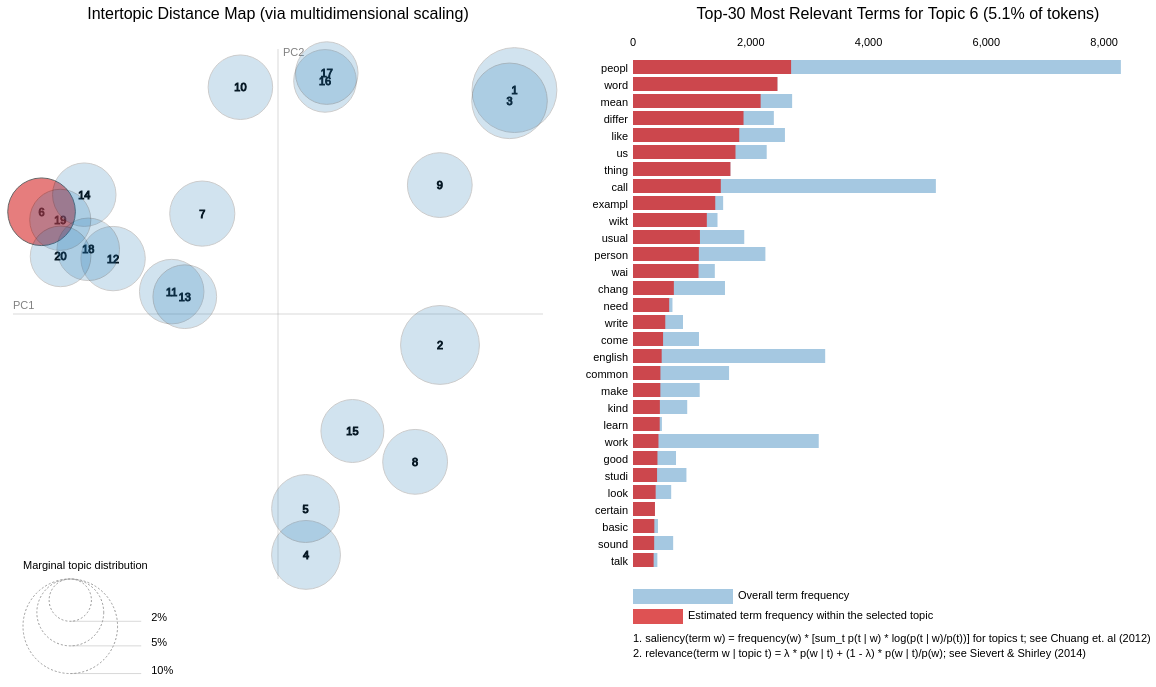
\includegraphics[width=.9\linewidth]{\gpath/m2t6.png}
 \end{subfigure}
 \caption{Plots of the first six topics}
 \label{fig:m2t56}
\end{figure}


%\begin{figure}
% \begin{subfigure}[c]{1\textwidth}
%  \caption{Topic 1}
%  \centering
%  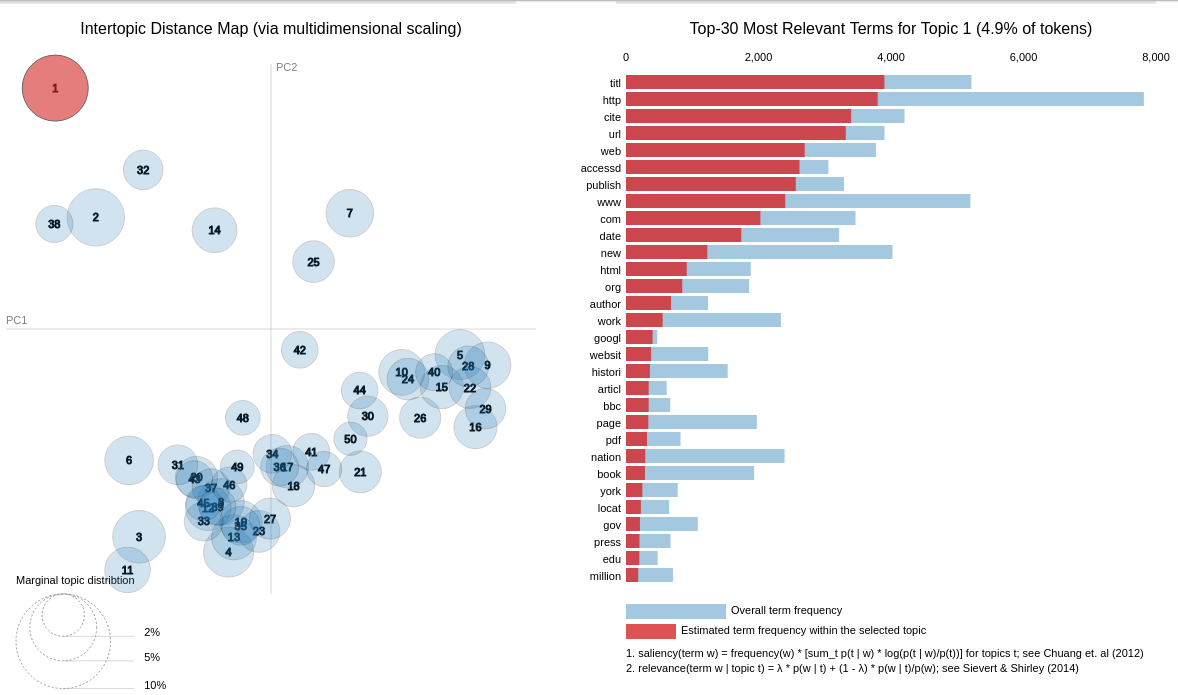
\includegraphics[width=.9\linewidth]{\gpath/t1.png}
% \end{subfigure}
% \begin{subfigure}[c]{1\textwidth}
%  \caption{Topic 2}
%  \centering
%  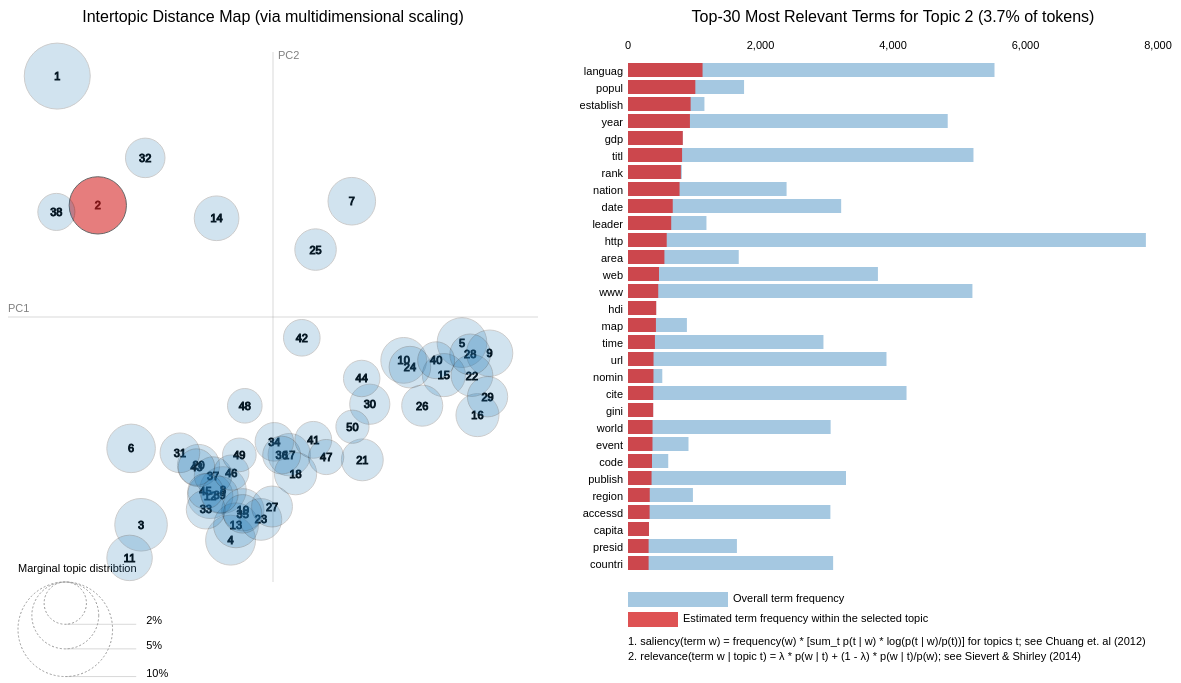
\includegraphics[width=.9\linewidth]{\gpath/t2.png}
% \end{subfigure}
% \caption{Plots of the first six topics}
% \label{fig:t12}
%\end{figure}
%
%
%\begin{figure}
% p\begin{subfigure}[c]{1\textwidth}
%  \caption{Topic 3}
%  \centering
%  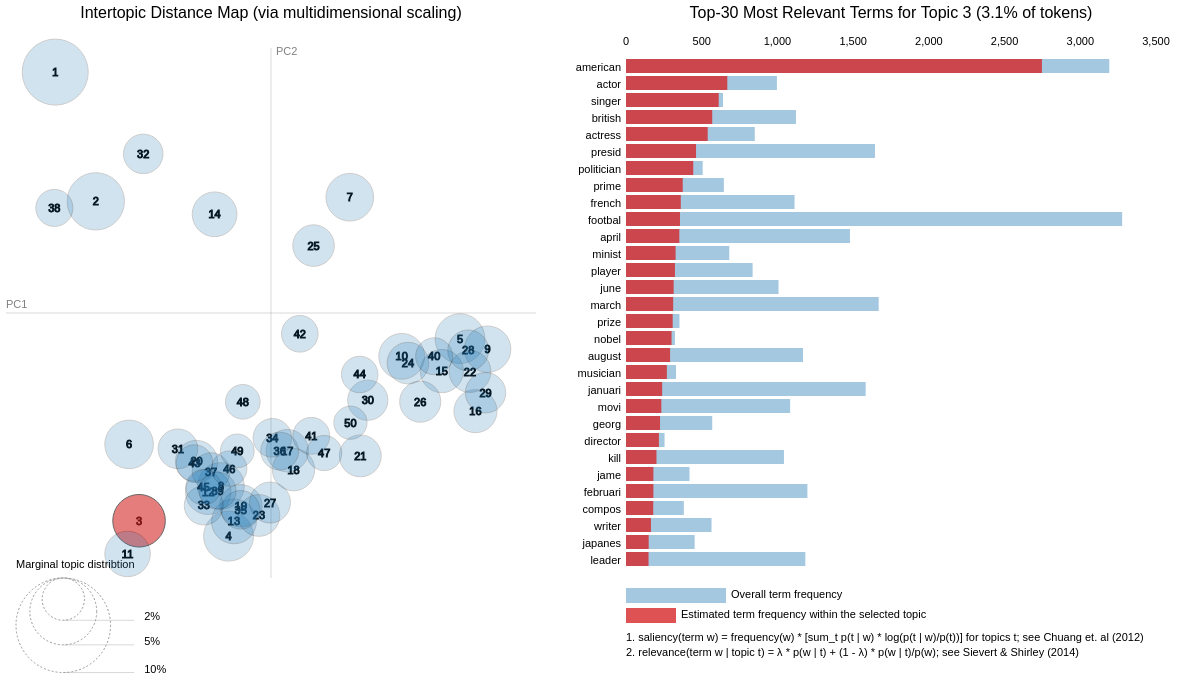
\includegraphics[width=.9\linewidth]{\gpath/t3.png}
% \end{subfigure}
% \begin{subfigure}[c]{1\textwidth}
%  \caption{Topic 4}
%  \centering
%  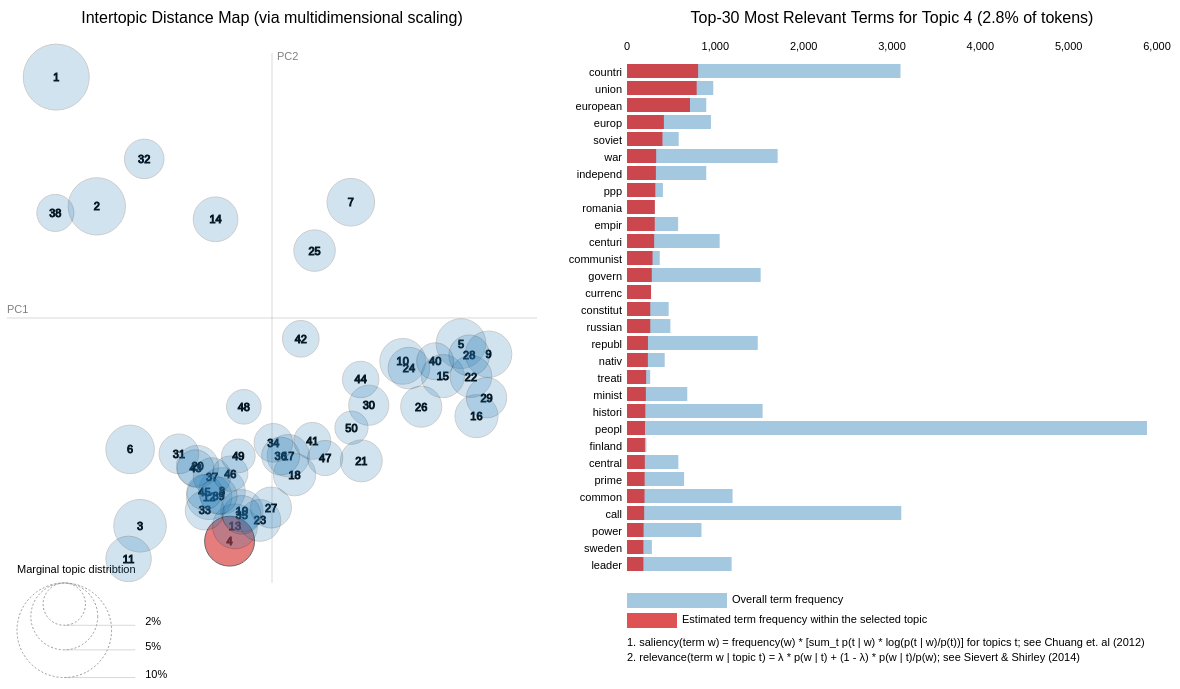
\includegraphics[width=.9\linewidth]{\gpath/t4.png}
% \end{subfigure}
% \caption{Plots of topic 3 and 4}
% \label{fig:t34}
%\end{figure}
%
%
%\begin{figure}
% p\begin{subfigure}[c]{1\textwidth}
%  \caption{Topic 5}
%  \centering
%  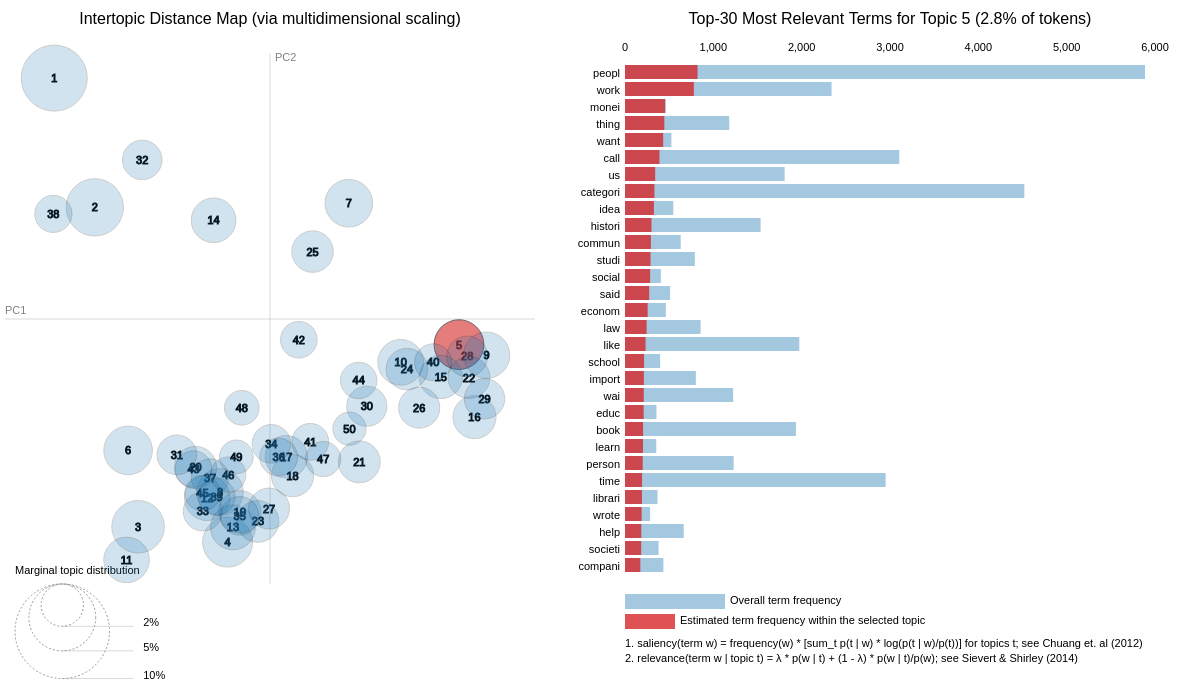
\includegraphics[width=.9\linewidth]{\gpath/t5.png}
% \end{subfigure}
% \begin{subfigure}[c]{1\textwidth}
%  \caption{Topic 6}
%  \centering
%  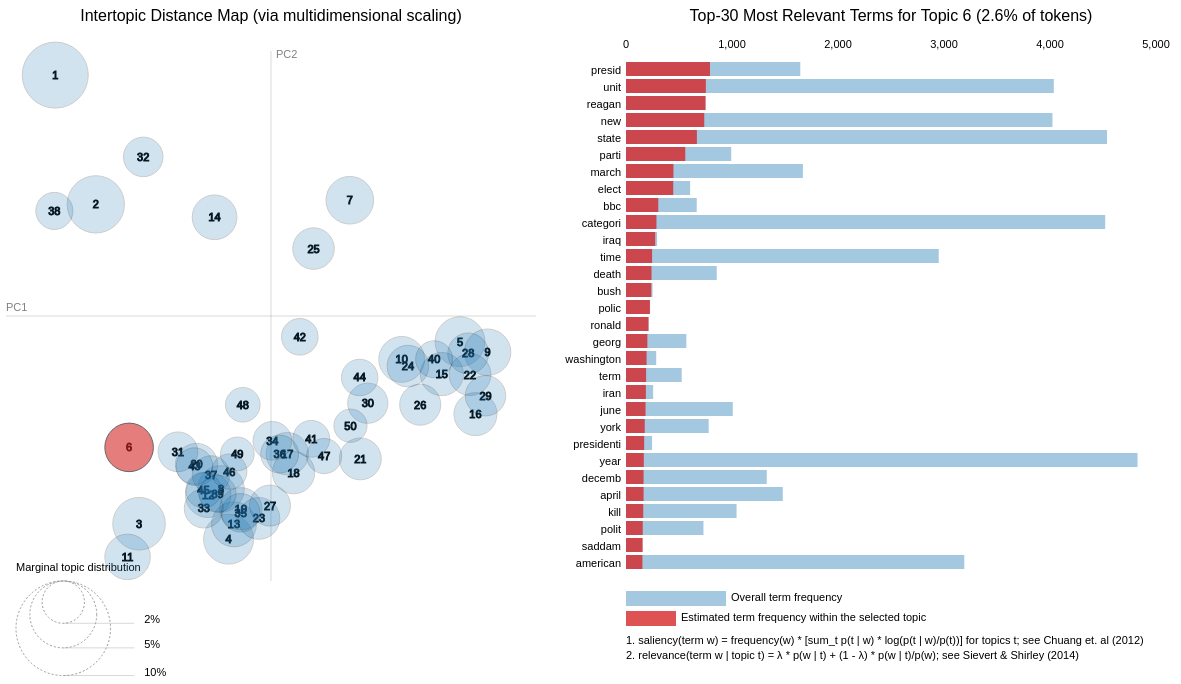
\includegraphics[width=.9\linewidth]{\gpath/t6.png}
% \end{subfigure}
% \caption{Plots of the first six topics}
% \label{fig:t56}
%\end{figure}




\newpage

\bibliography{refs}
\bibliographystyle{IEEEtran}

\newpage
%\onecolumn
\section{Appendix}
\subsection{Extract subset} \label{extract}
\lstinputlisting[language=bash]{\scriptpath/extractSmallSubset.bash}

\subsection{Class : Dataset} \label{class:dataset}
\lstinputlisting[language=python]{\codepath/lda/dataset.py}

\subsection{Class : LDA} \label{class:lda}
\lstinputlisting[language=python]{\codepath/lda/inference.py}

\subsection{Class : LDA} \label{code:generativeModel}
\lstinputlisting[language=python]{\codepath/lda/generativeModel.py}


\end{document}
